\section{第 10 章综合习题}

\begin{problem}{符号函数二重积分}{Sgn-Double-Integral}
    计算二重积分 $I = \iint_{D} \operatorname{sgn}(x^2 - y^2 + 2) \d x \d y$，其中 $D = \{(x, y) : x^2 + y^2 \le 4\}$．
\end{problem}

\begin{solution}
    根据符号函数的定义，令 $D_1 = \{(x, y) \in D : x^2 - y^2 + 2 \ge 0\}$，$D_2 = \{(x, y) \in D : x^2 - y^2 + 2 < 0\}$．则有
    \begin{equation}
        I = \iint_{D_1} 1 \d A - \iint_{D_2} 1 \d A = \operatorname{Area}(D_1) - \operatorname{Area}(D_2).
    \end{equation}
    由于 $\operatorname{Area}(D_1) + \operatorname{Area}(D_2) = \operatorname{Area}(D) = 4\uppi$，故
    \begin{equation}
        I = 4\uppi - 2\operatorname{Area}(D_2).
    \end{equation}
    区域 $D_2$ 由双曲线 $y^2 - x^2 = 2$ 在圆 $x^2 + y^2 = 4$ 内部的部分组成．联立方程
    \begin{equation}
        \begin{dcases}
            x^2 + y^2 = 4, \\
            y^2 - x^2 = 2.
        \end{dcases} \implies y^2 = 3, \ x^2 = 1.
    \end{equation}
    交点为 $(\pm 1, \pm \sqrt{3})$．$D_2$ 包含上下两个对称部分，其面积为
    \begin{equation}
        \operatorname{Area}(D_2) = 2 \int_{-1}^1 \left( \sqrt{4-x^2} - \sqrt{x^2+2} \right) \d x.
    \end{equation}
    分别计算其中的积分：
    \begin{equation}
        \begin{aligned}
            \int_{-1}^1 \sqrt{4-x^2} \d x & = \left[ \frac{x}{2}\sqrt{4-x^2} + 2\arcsin \frac{x}{2} \right]_{-1}^1 = \sqrt{3} + \frac{2\uppi}{3}, \\
            \int_{-1}^1 \sqrt{x^2+2} \d x & = \left[ \frac{x}{2}\sqrt{x^2+2} + \ln(x + \sqrt{x^2+2}) \right]_{-1}^1 = \sqrt{3} + \ln(2+\sqrt{3}).
        \end{aligned}
    \end{equation}
    从而得到
    \begin{equation}
        \operatorname{Area}(D_2) = 2 \left( \frac{2\uppi}{3} - \ln(2+\sqrt{3}) \right) = \frac{4\uppi}{3} - 2\ln(2+\sqrt{3}).
    \end{equation}
    代入 $I$ 的表达式：
    \begin{equation}
        I = 4\uppi - 2 \left( \frac{4\uppi}{3} - 2\ln(2+\sqrt{3}) \right) = \frac{4\uppi}{3} + 4\ln(2+\sqrt{3}).
    \end{equation}

    \begin{center}
        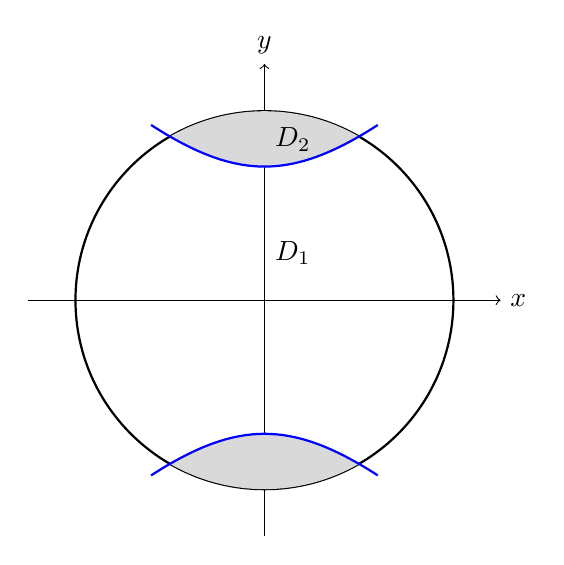
\begin{tikzpicture}[scale=1.2]
            \draw[->] (-2.5,0) -- (2.5,0) node[right] {$x$};
            \draw[->] (0,-2.5) -- (0,2.5) node[above] {$y$};
            \draw[thick] (0,0) circle (2);
            \fill[gray!30, domain=-1:1, samples=50]
            plot (\x, {sqrt(\x*\x+2)}) -- plot[domain=1:-1] (\x, {sqrt(4-\x*\x)}) -- cycle;
            \fill[gray!30, domain=-1:1, samples=50]
            plot (\x, {-sqrt(\x*\x+2)}) -- plot[domain=1:-1] (\x, {-sqrt(4-\x*\x)}) -- cycle;
            \draw[thick, blue, domain=-1.2:1.2, samples=50] plot (\x, {sqrt(\x*\x+2)});
            \draw[thick, blue, domain=-1.2:1.2, samples=50] plot (\x, {-sqrt(\x*\x+2)});
            \node at (0.3, 1.7) {$D_2$};
            \node at (0.3, 0.5) {$D_1$};
        \end{tikzpicture}
    \end{center}

    \begin{equation}
        \boxed{I = \frac{4\uppi}{3} + 4\ln(2+\sqrt{3})}
    \end{equation}
\end{solution}

\begin{problem}{三重积分计算}{Triple-Integral-Cube}
    计算三重积分
    \begin{equation}
        I = \iiint_{[0,1]^3} \frac{\d u \d v \d w}{(1 + u^2 + v^2 + w^2)^2}.
    \end{equation}
\end{problem}

\begin{solution}
    利用被积函数的对称性，可以将积分区域分解为三个相等的部分，分别对应 $u, v, w$ 为最大值的情况．
    \begin{equation}
        I = 3 \iiint_{0 \le v \le u, 0 \le w \le u, 0 \le u \le 1} \frac{\d u \d v \d w}{(1 + u^2 + v^2 + w^2)^2}.
    \end{equation}
    令 $v = ux$、$w = uy$，对应的 Jacobian 行列式为 $u^2$，积分变为
    \begin{equation}
        \begin{aligned}
            I & = 3 \int_0^1 \d x \int_0^1 \d y \int_0^1 \frac{u^2 \d u}{(1 + u^2(1 + x^2 + y^2))^2}                                                                      \\
              & = 3 \int_0^1 \int_0^1 \left[ \frac{1}{2(1+x^2+y^2)^{3/2}} \left( \arctan \sqrt{1+x^2+y^2} - \frac{\sqrt{1+x^2+y^2}}{2+x^2+y^2} \right) \right] \d x \d y.
        \end{aligned}
    \end{equation}
    将二重积分转换为极坐标 $x = r \cos \theta$、$y = r \sin \theta$，利用区域关于直线 $y = x$ 的对称性，取 $\theta \in [0, \uppi/4]$ 区域的两倍：
    \begin{equation}
        I = 3 \int_0^{\uppi/4} \d \theta \int_0^{( \cos \theta )^{-1}} \frac{r}{(1+r^2)^{3/2}} \left( \arctan \sqrt{1+r^2} - \frac{\sqrt{1+r^2}}{2+r^2} \right) \d r.
    \end{equation}
    令 $t = \sqrt{1+r^2}$，则 $r \d r = t \d t$．当 $r = 0$ 时 $t = 1$；当 $r = \sec \theta$ 时 $t = \sqrt{2 + \tan^2 \theta}$．积分化为
    \begin{equation}
        \begin{aligned}
            I & = 3 \int_0^{\uppi/4} \d \theta \int_1^{\sqrt{2 + \tan^2 \theta}} \left( \frac{\arctan t}{t^2} - \frac{1}{t(1+t^2)} \right) \d t    \\
              & = 3 \int_0^{\uppi/4} \left[ -\frac{\arctan t}{t} \right]_1^{\sqrt{2 + \tan^2 \theta}} \d \theta                                    \\
              & = 3 \int_0^{\uppi/4} \left( \frac{\uppi}{4} - \frac{\arctan \sqrt{2 + \tan^2 \theta}}{\sqrt{2 + \tan^2 \theta}} \right) \d \theta.
        \end{aligned}
    \end{equation}
    设 $J = \int_0^{\uppi/4} \frac{\arctan \sqrt{2 + \tan^2 \theta}}{\sqrt{2 + \tan^2 \theta}} \d \theta$．令 $\tan \theta = z$，则 $\d \theta = \frac{\d z}{1+z^2}$，
    \begin{equation}
        J = \int_0^1 \frac{\arctan \sqrt{2+z^2}}{(1+z^2)\sqrt{2+z^2}} \d z.
    \end{equation}
    再考虑积分 $K = \int_0^1 \frac{\arctan (1/\sqrt{2+z^2})}{(1+z^2)\sqrt{2+z^2}} \d z$．利用恒等式 $\frac{\arctan (1/A)}{A} = \int_0^1 \frac{\d y}{A^2 + y^2}$ 可知
    \begin{equation}
        K = \int_0^1 \int_0^1 \frac{\d y \d z}{(1+z^2)(2+z^2+y^2)} = \int_0^1 \frac{1}{1+y^2} \left[ \frac{\uppi}{4} - \frac{\arctan (1/\sqrt{2+y^2})}{\sqrt{2+y^2}} \right] \d y = \frac{\uppi^2}{16} - K.
    \end{equation}
    由此解得 $K = \frac{\uppi^2}{32}$．利用 $J + K = \int_0^1 \frac{\uppi/2}{(1+z^2)\sqrt{2+z^2}} \d z = \frac{\uppi}{2} \cdot \frac{\uppi}{6} = \frac{\uppi^2}{12}$，可求得 $J = \frac{5\uppi^2}{96}$．代入原式得
    \begin{equation}
        I = \frac{3 \uppi^2}{16} - 3 \cdot \frac{5\uppi^2}{96} = \frac{18\uppi^2 - 15\uppi^2}{96} = \frac{3\uppi^2}{96} = \frac{\uppi^2}{32}.
    \end{equation}
    \begin{equation}
        \boxed{I = \frac{\uppi^2}{32}}
    \end{equation}
\end{solution}

\begin{note}{一个更巧妙的解法}{A-Smarter-Solution}
    {\kaishu 上述解法思路简单，但计算稍显复杂，实际上还有一个技巧性更强的解法如下：}
    \begin{solution}
        利用积分恒等式 $\frac{1}{A^2} = \int_{0}^{\infty} t \e^{-At} \d{t}$，令 $A = 1 + x^2 + y^2 + z^2$，则有
        \begin{equation}
            \begin{aligned}
                I & = \iiint_{[0,1]^3} \left( \int_{0}^{\infty} t \e^{-(1+x^2+y^2+z^2)t} \d{t} \right) \d{x} \d{y} \d{z}                                                                          \\
                  & = \int_{0}^{\infty} t \e^{-t} \left( \int_{0}^{1} \e^{-x^2 t} \d{x} \right) \left( \int_{0}^{1} \e^{-y^2 t} \d{y} \right) \left( \int_{0}^{1} \e^{-z^2 t} \d{z} \right) \d{t} \\
                  & = \int_{0}^{\infty} t \e^{-t} \left( \int_{0}^{1} \e^{-x^2 t} \d{x} \right)^3 \d{t}.
            \end{aligned}
        \end{equation}
        在内层积分中令 $u = x\sqrt{t}$，则 $\d{x} = \frac{1}{\sqrt{t}} \d{u}$，代入上式得
        \begin{equation}
            \begin{aligned}
                I & = \int_{0}^{\infty} t \e^{-t} \left( \int_{0}^{\sqrt{t}} \e^{-u^2} \frac{1}{\sqrt{t}} \d{u} \right)^3 \d{t} \\
                  & = \int_{0}^{\infty} \frac{1}{\sqrt{t}} \e^{-t} \left( \int_{0}^{\sqrt{t}} \e^{-u^2} \d{u} \right)^3 \d{t}.
            \end{aligned}
        \end{equation}
        注意到 $\d \left( \int_{0}^{\sqrt{t}} \e^{-u^2} \d{u} \right) = \frac{\e^{-t}}{2\sqrt{t}} \d{t}$，故
        \begin{equation}
            I = 2 \int_{0}^{\infty} \left( \int_{0}^{\sqrt{t}} \e^{-u^2} \d{u} \right)^3 \d \left( \int_{0}^{\sqrt{t}} \e^{-u^2} \d{u} \right). \label{eq:Integral-Form}
        \end{equation}
        由于 $\int_{0}^{\infty} \e^{-u^2} \d{u} = \frac{\sqrt{\uppi}}{2}$，对 \zcref{eq:Integral-Form} 进行积分计算得
        \begin{equation}
            I = 2 \left[ \frac{1}{4} \left( \int_{0}^{\sqrt{t}} \e^{-u^2} \d{u} \right)^4 \right]_{0}^{\infty} = \frac{1}{2} \left( \frac{\sqrt{\uppi}}{2} \right)^4.
        \end{equation}
        整理得最终结果为
        \begin{equation}
            \boxed{I = \frac{\uppi^2}{32}}.
        \end{equation}
    \end{solution}

\end{note}

\begin{problem}{含参变量积分}{Parametric-Integral}
    设 $a > 0, b > 0$．试求下面的积分：
    \begin{enumerate}
        \item $I_1 = \int_0^1 \sin \left( \ln \frac{1}{x} \right) \cdot \frac{x^b - x^a}{\ln x} \d x$；
        \item $I_2 = \int_0^1 \cos \left( \ln \frac{1}{x} \right) \cdot \frac{x^b - x^a}{\ln x} \d x$．
    \end{enumerate}
\end{problem}

\begin{solution}
    \ansitem{1}
    利用恒等式 $\frac{x^b - x^a}{\ln x} = \int_a^b x^y \d y$．作代换 $u = \ln \frac{1}{x}$，则 $x = \e^{-u}$，$\d x = -\e^{-u} \d u$．当 $x = 0$ 时，$u \to +\infty$；当 $x = 1$ 时，$u = 0$．
    \begin{equation}
        \begin{aligned}
            I_1 & = \int_0^\infty \sin u \cdot \left( \int_a^b \e^{-uy} \d y \right) \e^{-u} \d u \\
                & = \int_a^b \left( \int_0^\infty \e^{-(y+1)u} \sin u \d u \right) \d y.
        \end{aligned}
    \end{equation}
    注意到内部积分是基本的指数与三角函数乘积积分，由于 $y+1 > 0$，有
    \begin{equation}
        \int_0^\infty \e^{-(y+1)u} \sin u \d u = \left. \frac{\e^{-(y+1)u} [-(y+1) \sin u - \cos u]}{(y+1)^2 + 1} \right|_0^\infty = \frac{1}{(y+1)^2 + 1}.
    \end{equation}
    代回原式得
    \begin{equation}
        I_1 = \int_a^b \frac{1}{(y+1)^2 + 1} \d y = \arctan(y+1) \Big|_a^b.
    \end{equation}
    最终结果为
    \begin{equation}
        \boxed{I_1 = \arctan(b+1) - \arctan(a+1)}
    \end{equation}

    \ansitem{2}
    同理，对 $I_2$ 使用相同的变量代换并交换积分次序
    \begin{equation}
        I_2 = \int_a^b \left( \int_0^\infty \e^{-(y+1)u} \cos u \d u \right) \d y.
    \end{equation}
    计算内部积分
    \begin{equation}
        \int_0^\infty \e^{-(y+1)u} \cos u \d u = \left. \frac{\e^{-(y+1)u} [-(y+1) \cos u + \sin u]}{(y+1)^2 + 1} \right|_0^\infty = \frac{y+1}{(y+1)^2 + 1}.
    \end{equation}
    带入计算得
    \begin{equation}
        I_2 = \int_a^b \frac{y+1}{(y+1)^2 + 1} \d y = \frac{1}{2} \ln \left[ (y+1)^2 + 1 \right] \Big|_a^b.
    \end{equation}
    最终结果为
    \begin{equation}
        \boxed{I_2 = \frac{1}{2} \ln \frac{(b+1)^2 + 1}{(a+1)^2 + 1}}
    \end{equation}
\end{solution}

\begin{problem}{二重积分}{Double-Integral}
    设 $D = \{(x, y) \mid x^2 + y^2 \le 1\}$．求 $I = \iint_D \left| \frac{x+y}{\sqrt{2}} - x^2 - y^2 \right| \d x \d y$．
\end{problem}

\begin{solution}
    引入极坐标 $x = r \cos \theta$、$y = r \sin \theta$，其雅可比行列式为 $r$．原积分可化为
    \begin{equation}
        \begin{aligned}
            I & = \int_0^{2\uppi} \d \theta \int_0^1 \left| \frac{r(\cos \theta + \sin \theta)}{\sqrt{2}} - r^2 \right| r \d r   \\
              & = \int_0^{2\uppi} \d \theta \int_0^1 \left| r \sin \left( \theta + \frac{\uppi}{4} \right) - r^2 \right| r \d r.
        \end{aligned}
    \end{equation}
    利用被积函数关于 $\theta$ 的 $2\uppi$ 周期性，令 $\alpha = \theta + \frac{\uppi}{4}$，则有
    \begin{equation}
        I = \int_0^{2\uppi} \d \alpha \int_0^1 r^2 |\sin \alpha - r| \d r. \label{eq:Integral-Form-2}
    \end{equation}
    设内层积分为 $f(\alpha)$，分情况讨论如下：
    当 $\sin \alpha \le 0$ 时，即 $\alpha \in [\uppi, 2\uppi]$，有
    \begin{equation}
        f(\alpha) = \int_0^1 r^2 (r - \sin \alpha) \d r = \frac{1}{4} - \frac{1}{3} \sin \alpha.
    \end{equation}
    当 $\sin \alpha > 0$ 时，即 $\alpha \in [0, \uppi]$，有
    \begin{equation}
        f(\alpha) = \int_0^{\sin \alpha} r^2 (\sin \alpha - r) \d r + \int_{\sin \alpha}^1 r^2 (r - \sin \alpha) \d r = \frac{1}{6} \sin^4 \alpha - \frac{1}{3} \sin \alpha + \frac{1}{4}.
    \end{equation}
    将上述结果代入 \zcref{eq:Integral-Form-2} 进行计算：
    \begin{equation}
        \begin{aligned}
            I & = \int_0^{\uppi} \left( \frac{1}{6} \sin^4 \alpha - \frac{1}{3} \sin \alpha + \frac{1}{4} \right) \d \alpha + \int_{\uppi}^{2\uppi} \left( \frac{1}{4} - \frac{1}{3} \sin \alpha \right) \d \alpha \\
              & = \left( \frac{1}{6} \cdot \frac{3\uppi}{8} - \frac{2}{3} + \frac{\uppi}{4} \right) + \left( \frac{\uppi}{4} + \frac{2}{3} \right)                                                                 \\
              & = \frac{\uppi}{16} + \frac{\uppi}{2}                                                                                                                                                               \\
              & = \frac{9\uppi}{16}.
        \end{aligned}
    \end{equation}
    \begin{equation}
        \boxed{I = \frac{9\uppi}{16}}
    \end{equation}
\end{solution}

\begin{problem}{二重积分的应用与极坐标面积}{Lemniscate-Circle-Intersection}
    试求圆盘 $(x-a)^2 + (y-a)^2 \le a^2$ 与曲线 $(x^2 + y^2)^2 = 8a^2 xy$ 所围部分相交的区域 $D$ 的面积．
\end{problem}

\begin{solution}
    建立极坐标系 $x = r \cos \theta, y = r \sin \theta$．圆盘的边界方程可化为
    \begin{equation}
        (r \cos \theta - a)^2 + (r \sin \theta - a)^2 = a^2 \implies r^2 - 2ar(\cos \theta + \sin \theta) + a^2 = 0
    \end{equation}
    解得圆盘在第一象限的内外边界极半径分别为
    \begin{equation}
        r = a(\cos \theta + \sin \theta) \pm a \sqrt{(\cos \theta + \sin \theta)^2 - 1} = a(\cos \theta + \sin \theta) \pm a \sqrt{\sin 2\theta}
    \end{equation}
    曲线 $(x^2 + y^2)^2 = 8a^2 xy$ 即伯努利双纽线，其极坐标方程为
    \begin{equation}
        r^2 = 4a^2 \sin 2\theta \implies r = 2a \sqrt{\sin 2\theta}
    \end{equation}
    根据题意，区域 $D$ 是圆盘内部与双纽线内部的交集．由于双纽线在第一象限的部分满足 $r \le 2a\sqrt{\sin 2\theta}$，而圆盘内部满足 $a(\cos \theta + \sin \theta) - a \sqrt{\sin 2\theta} \le r \le a(\cos \theta + \sin \theta) + a \sqrt{\sin 2\theta}$．令两曲线边界相交，有
    \begin{equation}
        2a\sqrt{\sin 2\theta} = a(\cos \theta + \sin \theta) - a\sqrt{\sin 2\theta} \implies 3\sqrt{\sin 2\theta} = \sqrt{1 + \sin 2\theta}
    \end{equation}
    平方得 $9\sin 2\theta = 1 + \sin 2\theta$，即 $\sin 2\theta = \frac{1}{8}$．设 $\alpha = \frac{1}{2} \arcsin \frac{1}{8}$，则积分范围为 $\theta \in [\alpha, \frac{\uppi}{2} - \alpha]$．在该范围内，$r$ 的取值区间为 $[a(\cos \theta + \sin \theta) - a\sqrt{\sin 2\theta}, 2a\sqrt{\sin 2\theta}]$．

    由对称性，令 $\theta = \varphi + \frac{\uppi}{4}$，则 $\varphi \in [-\varphi_0, \varphi_0]$，其中 $\cos 2\varphi_0 = \frac{1}{8}$．此时 $\sin 2\theta = \cos 2\varphi$，$\cos \theta + \sin \theta = \sqrt{2} \cos \varphi$．区域面积为
    \begin{equation}
        \begin{aligned}
            S & = \int_{\alpha}^{\frac{\uppi}{2}-\alpha} \d \theta \int_{a(\cos\theta+\sin\theta)-a\sqrt{\sin2\theta}}^{2a\sqrt{\sin2\theta}} r \d r     \\
              & = \frac{a^2}{2} \int_{-\varphi_0}^{\varphi_0} \left[ 4 \cos 2\varphi - (\sqrt{2}\cos\varphi - \sqrt{\cos 2\varphi})^2 \right] \d \varphi \\
              & = a^2 \int_{-\varphi_0}^{\varphi_0} \left( \cos 2\varphi - \frac{1}{2} + \sqrt{2}\cos\varphi\sqrt{\cos 2\varphi} \right) \d \varphi
        \end{aligned}
    \end{equation}
    计算各项积分：
    \begin{equation}
        \int_{-\varphi_0}^{\varphi_0} \left( \cos 2\varphi - \frac{1}{2} \right) \d \varphi = \sin 2\varphi_0 - \varphi_0 = \frac{3\sqrt{7}}{8} - \arcsin \frac{\sqrt{7}}{4}
    \end{equation}
    对于最后一项，令 $\sqrt{2}\sin\varphi = \sin t$，则 $\sqrt{2}\cos\varphi \d \varphi = \cos t \d t$．当 $\varphi = \varphi_0$ 时，$t_0 = \arcsin(\sqrt{2}\sin\varphi_0) = \arcsin\frac{\sqrt{14}}{4}$．
    \begin{equation}
        \int_{-\varphi_0}^{\varphi_0} \sqrt{2}\cos\varphi\sqrt{\cos 2\varphi} \d \varphi = \int_{-t_0}^{t_0} \cos^2 t \d t = t_0 + \sin t_0 \cos t_0 = \arcsin\frac{\sqrt{14}}{4} + \frac{\sqrt{7}}{8}
    \end{equation}
    综上所述，区域 $D$ 的面积为
    \begin{equation}
        S =  a^2 \left( \frac{\sqrt{7}}{2} + \arcsin \frac{\sqrt{14}}{4} - \arcsin \frac{\sqrt{7}}{4} \right) = \boxed{a^2 \left( \frac{\sqrt{7}}{2} + \arcsin \frac{\sqrt{14}}{8} \right) }
    \end{equation}

    \begin{center}
        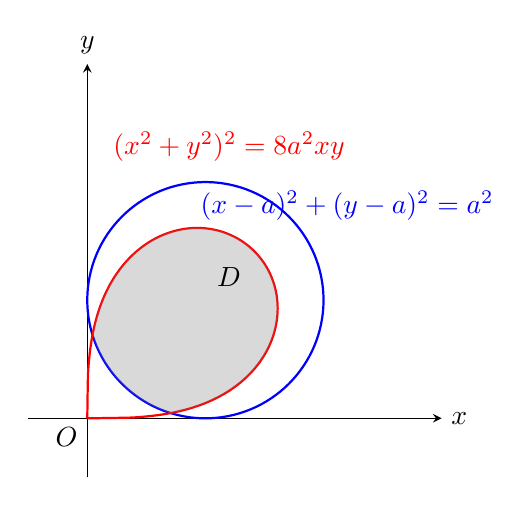
\begin{tikzpicture}[scale=1.5, >=stealth]
            \draw[->] (-0.5,0) -- (3,0) node[right] {$x$};
            \draw[->] (0,-0.5) -- (0,3) node[above] {$y$};
            \draw (0,0) node[below left] {$O$};

            % Circle (a=1)
            \draw[thick, blue] (1,1) circle (1);
            \node[blue] at (2.2,1.8) {$(x-a)^2+(y-a)^2=a^2$};

            % Lemniscate
            \draw[thick, red, domain=0:90, samples=100, smooth] plot ( {2*sqrt(sin(2*\x))*cos(\x)}, {2*sqrt(sin(2*\x))*sin(\x)} );
            \node[red] at (1.2,2.3) {$(x^2+y^2)^2=8a^2xy$};

            % Intersection area shading (approximate for visualization)
            \fill[gray, opacity=0.3, domain=3.59:86.41, samples=100]
            plot ( {2*sqrt(sin(2*\x))*cos(\x)}, {2*sqrt(sin(2*\x))*sin(\x)} ) --
            plot[domain=86.41:3.59] ( {(cos(\x)+sin(\x)-sqrt(sin(2*\x)))*cos(\x)}, {(cos(\x)+sin(\x)-sqrt(sin(2*\x)))*sin(\x)} ) -- cycle;
            \node at (1.2,1.2) {$D$};
        \end{tikzpicture}
    \end{center}
\end{solution}

\begin{problem}{三重积分计算体积}{Volume-Spherical-Coordinates}
    计算曲面 $(x^2 + y^2)^2 + z^4 = y$ 所围的体积 $V$．
\end{problem}

\begin{solution}
    引入球坐标变换
    \begin{equation}
        x = r \sin \theta \cos \varphi, \quad y = r \sin \theta \sin \varphi, \quad z = r \cos \theta,
    \end{equation}
    其中 $r \ge 0$、$\theta \in [0, \uppi]$、$\varphi \in [0, 2\uppi]$，雅可比行列式为 $r^2 \sin \theta$．将变换代入曲面方程得
    \begin{equation}
        (r^2 \sin^2 \theta)^2 + (r \cos \theta)^4 = r \sin \theta \sin \varphi,
    \end{equation}
    整理得
    \begin{equation}
        \label{eq:rho-theta-phi}
        r^3 = \frac{\sin \theta \sin \varphi}{\sin^4 \theta + \cos^4 \theta}.
    \end{equation}
    由于 $r \ge 0$ 且 $\sin \theta \ge 0$，由 \zcref{eq:rho-theta-phi} 可知 $\sin \varphi \ge 0$，故 $\varphi \in [0, \uppi]$．体积 $V$ 为
    \begin{equation}
        \begin{aligned}
            V & = \int_{0}^{\uppi} \d \varphi \int_{0}^{\uppi} \d \theta \int_{0}^{\sqrt[3]{\frac{\sin \theta \sin \varphi}{\sin^4 \theta + \cos^4 \theta}}} r^2 \sin \theta \d r    \\
              & = \frac{1}{3} \int_{0}^{\uppi} \d \varphi \int_{0}^{\uppi} \frac{\sin^2 \theta \sin \varphi}{\sin^4 \theta + \cos^4 \theta} \d \theta                                \\
              & = \frac{1}{3} \left( \int_{0}^{\uppi} \sin \varphi \d \varphi \right) \left( \int_{0}^{\uppi} \frac{\sin^2 \theta}{\sin^4 \theta + \cos^4 \theta} \d \theta \right).
        \end{aligned}
    \end{equation}
    计算第一个积分
    \begin{equation}
        \int_{0}^{\uppi} \sin \varphi \d \varphi = \left[ -\cos \varphi \right]_{0}^{\uppi} = 2.
    \end{equation}
    对于第二个积分，利用对称性有
    \begin{equation}
        \int_{0}^{\uppi} \frac{\sin^2 \theta}{\sin^4 \theta + \cos^4 \theta} \d \theta = 2 \int_{0}^{\uppi/2} \frac{\sin^2 \theta}{\sin^4 \theta + \cos^4 \theta} \d \theta.
    \end{equation}
    分子分母同除以 $\cos^4 \theta$，令 $u = \tan \theta$，则 $\d u = \sec^2 \theta \d \theta$
    \begin{equation}
        2 \int_{0}^{\uppi/2} \frac{\tan^2 \theta \sec^2 \theta}{\tan^4 \theta + 1} \d \theta = 2 \int_{0}^{+\infty} \frac{u^2}{u^4 + 1} \d u.
    \end{equation}
    利用代换 $u = 1/t$ 可知 $\int_{0}^{+\infty} \frac{u^2}{u^4 + 1} \d u = \int_{0}^{+\infty} \frac{1}{t^4 + 1} \d t$，故
    \begin{equation}
        2 \int_{0}^{+\infty} \frac{u^2}{u^4 + 1} \d u = \int_{0}^{+\infty} \frac{u^2 + 1}{u^4 + 1} \d u = \int_{0}^{+\infty} \frac{1 + \frac{1}{u^2}}{u^2 + \frac{1}{u^2}} \d u = \int_{0}^{+\infty} \frac{\d (u - \frac{1}{u})}{(u - \frac{1}{u})^2 + 2}.
    \end{equation}
    令 $w = u - \frac{1}{u}$，积分变为
    \begin{equation}
        \int_{-\infty}^{+\infty} \frac{\d w}{w^2 + 2} = \left[ \frac{1}{\sqrt{2}} \arctan \frac{w}{\sqrt{2}} \right]_{-\infty}^{+\infty} = \frac{\uppi}{\sqrt{2}}.
    \end{equation}
    代回体积表达式得
    \begin{equation}
        V = \frac{1}{3} \cdot 2 \cdot \frac{\uppi}{\sqrt{2}} = \frac{\sqrt{2}\uppi}{3}.
    \end{equation}
    \begin{equation}
        \boxed{V = \frac{\sqrt{2}\uppi}{3}}
    \end{equation}
\end{solution}

\begin{problem}{变量替换与积分次序}{Double-Integral-Proof}
    证明：
    \begin{equation}
        \iint_{[0,1]^2} (xy)^{xy} \d x \d y = \int_0^1 t^t \d t.
    \end{equation}
\end{problem}

\begin{myproof}
    记 $I = \iint_{[0,1]^2} (xy)^{xy} \d x \d y$，将其写作累次积分形式
    \begin{equation}
        I = \int_0^1 \left( \int_0^1 (xy)^{xy} \d y \right) \d x.
    \end{equation}
    对于内层积分，固定 $x \in (0, 1]$，令 $u = xy$，则有 $y = \frac{u}{x}$ 且 $\d y = \frac{1}{x} \d u$．当 $y$ 从 $0$ 变到 $1$ 时，$u$ 从 $0$ 变到 $x$
    \begin{equation}
        I = \int_0^1 \left( \int_0^x u^u \frac{1}{x} \d u \right) \d x.
    \end{equation}
    由积分区域 $D = \{(u, x) \mid 0 \le u \le x \le 1\}$，交换积分次序可得
    \begin{equation}
        \begin{aligned}
            I & = \int_0^1 u^u \left( \int_u^1 \frac{1}{x} \d x \right) \d u \\
              & = \int_0^1 u^u \left[ \ln x \right]_u^1 \d u                 \\
              & = \int_0^1 u^u (-\ln u) \d u.
        \end{aligned}
    \end{equation}
    注意到 $\frac{\d}{\d u} (u^u) = \frac{\d}{\d u} (\e^{u \ln u}) = u^u (1 + \ln u)$，故有 $u^u \ln u = \frac{\d}{\d u} (u^u) - u^u$．代入上式得
    \begin{equation}
        \begin{aligned}
            I & = - \int_0^1 \left[ \frac{\d}{\d u} (u^u) - u^u \right] \d u \\
              & = - \left[ u^u \right]_0^1 + \int_0^1 u^u \d u.
        \end{aligned}
    \end{equation}
    利用极限 $\lim_{u \to 0^+} u^u = 1$，可得 $\left[ u^u \right]_0^1 = 1^1 - 1 = 0$．因此
    \begin{equation}
        \boxed{\iint_{[0,1]^2} (xy)^{xy} \d x \d y = \int_0^1 t^t \d t}
    \end{equation}
\end{myproof}

\begin{problem}{二重积分的换元法}{Substitution-Double-Integral}
    设 $a, b$ 是不全为 $0$ 的常数．求证：
    \begin{equation}
        \iint_{x^2+y^2 \le 1} f(ax+by+c) \d x \d y = 2 \int_{-1}^1 \sqrt{1-t^2} f \left( t \sqrt{a^2+b^2} + c \right) \d t.
    \end{equation}
\end{problem}

\begin{myproof}
    令 $L = \sqrt{a^2+b^2}$．作如下变量替换：
    \begin{equation}\label{eq:substitution}
        u = \frac{ax+by}{L},\quad v = \frac{-bx+ay}{L}.
    \end{equation}
    由此可得
    \begin{equation}\label{eq:uv-properties}
        u^2 + v^2 = \frac{(ax+by)^2 + (-bx+ay)^2}{L^2} = \frac{(a^2+b^2)x^2 + (a^2+b^2)y^2}{a^2+b^2} = x^2+y^2.
    \end{equation}
    相应的逆变换为
    \begin{equation}\label{eq:inverse-sub}
        x = \frac{au-bv}{L},\quad y = \frac{bu+av}{L}.
    \end{equation}
    计算该变换的雅可比行列式：
    \begin{equation}\label{eq:jacobian}
        \frac{\partial(x, y)}{\partial(u, v)} = \det \begin{bmatrix} \frac{a}{L} & -\frac{b}{L} \\ \frac{b}{L} & \frac{a}{L} \end{bmatrix} = \frac{a^2+b^2}{L^2} = 1.
    \end{equation}
    变换后，积分区域 $D = \{ (x,y) \mid x^2+y^2 \le 1 \}$ 变为 $D' = \{ (u,v) \mid u^2+v^2 \le 1 \}$．
    于是，原积分可化为
    \begin{equation}\label{eq:integration-process}
        \begin{aligned}
            \iint_{x^2+y^2 \le 1} f(ax+by+c) \d x \d y & = \iint_{u^2+v^2 \le 1} f(uL+c) \d u \d v                                          \\
                                                       & = \int_{-1}^1 \left( \int_{-\sqrt{1-u^2}}^{\sqrt{1-u^2}} \d v \right) f(uL+c) \d u \\
                                                       & = \int_{-1}^1 2 \sqrt{1-u^2} f \left( u \sqrt{a^2+b^2} + c \right) \d u.
        \end{aligned}
    \end{equation}
    记积分变量为 $t$，即得
    \begin{equation}
        \boxed{\iint_{x^2+y^2 \le 1} f(ax+by+c) \d x \d y = 2 \int_{-1}^1 \sqrt{1-t^2} f \left( t \sqrt{a^2+b^2} + c \right) \d t}
    \end{equation}
\end{myproof}

\begin{problem}{多元函数积分与微分}{Differentiation-of-Integral}
    设 $f$ 是连续可导的单变量函数．令 $F(t) = \iint_{[0,t]^2} f(xy) \, \d x \d y$．求证：
    \begin{enumerate}
        \item $F'(t) = \frac{2}{t} \left( F(t) + \iint_{[0,t]^2} xy f'(xy) \, \d x \d y \right)$；
        \item $F'(t) = \frac{2}{t} \int_{0}^{t^2} f(s) \, \d s$．
    \end{enumerate}
\end{problem}

\begin{myproof}
    \ansitem{1}
    通过作变量替换 $x = tu$，$y = tv$，其雅可比行列式为 $J = t^2$．积分区域从 $[0,t]^2$ 变为 $[0,1]^2$：
    \begin{equation}
        \begin{aligned}
            F(t) & = \int_0^1 \int_0^1 f(t^2 uv) \cdot t^2 \, \d u \d v \\
                 & = t^2 \int_0^1 \int_0^1 f(t^2 uv) \, \d u \d v.
        \end{aligned} \label{eq:F-t-form}
    \end{equation}
    对 \zcref{eq:F-t-form} 关于 $t$ 求导，根据含参变量积分求导法则：
    \begin{equation}
        \begin{aligned}
            F'(t) & = 2t \int_0^1 \int_0^1 f(t^2 uv) \, \d u \d v + t^2 \int_0^1 \int_0^1 f'(t^2 uv) \cdot 2t uv \, \d u \d v                                 \\
                  & = \frac{2}{t} \left( t^2 \int_0^1 \int_0^1 f(t^2 uv) \, \d u \d v + \int_0^1 \int_0^1 (t^2 uv) f'(t^2 uv) \cdot t^2 \, \d u \d v \right).
        \end{aligned}
    \end{equation}
    逆向使用变量替换 $x = tu$，$y = tv$，即得：
    \begin{equation}
        \boxed{F'(t) = \frac{2}{t} \left( F(t) + \iint_{[0,t]^2} xy f'(xy) \, \d x \d y \right)}
    \end{equation}

    \ansitem{2}
    考虑 \zcref{eq:F-t-form} 中的第二项积分 $I = \iint_{[0,t]^2} xy f'(xy) \, \d x \d y$．利用累次积分：
    \begin{equation}
        I = \int_0^t \left( \int_0^t x f'(xy) \, \d y \right) x \, \d x.
    \end{equation}
    对内层关于 $y$ 的积分使用分部积分法，令 $u = xy$，$ \d u = x \d y$：
    \begin{equation}
        \begin{aligned}
            \int_0^t x f'(xy) \, \d y & = \int_0^{xt} f'(u) \, \d u \\
                                      & = f(xt) - f(0).
        \end{aligned}
    \end{equation}
    故 $I = \int_0^t x f(xt) \, \d x - \int_0^t x f(0) \, \d x$．此法稍显繁琐，采用直接对原积分进行降维处理．

    令 $F(t) = \int_0^t \left( \int_0^t f(xy) \, \d x \right) \d y$．对内层积分令 $s = xy$，则 $\d x = \frac{1}{y} \d s$：
    \begin{equation}
        F(t) = \int_0^t \frac{1}{y} \left( \int_0^{ty} f(s) \, \d s \right) \d y.
    \end{equation}
    对 $t$ 求导，根据莱布尼茨公式：
    \begin{equation}
        \begin{aligned}
            F'(t) & = \left[ \frac{1}{y} \int_0^{ty} f(s) \, \d s \right]_{y=t} + \int_0^t \frac{\partial}{\partial t} \left( \frac{1}{y} \int_0^{ty} f(s) \, \d s \right) \d y \\
                  & = \frac{1}{t} \int_0^{t^2} f(s) \, \d s + \int_0^t \frac{1}{y} f(ty) y \, \d y                                                                              \\
                  & = \frac{1}{t} \int_0^{t^2} f(s) \, \d s + \int_0^t f(ty) \, \d y.
        \end{aligned}
    \end{equation}
    对于最后一项积分，令 $u = ty$，则 $\d y = \frac{1}{t} \d u$：
    \begin{equation}
        \int_0^t f(ty) \, \d y = \frac{1}{t} \int_0^{t^2} f(u) \, \d u.
    \end{equation}
    综上所述：
    \begin{equation}
        \boxed{F'(t) = \frac{2}{t} \int_0^{t^2} f(s) \, \d s}
    \end{equation}
\end{myproof}


\begin{problem}{Poincaré 不等式}{Poincare-Inequality}
    设 $\varphi(x), \psi(x)$ 是 $[a, b]$ 上的连续函数，$f(x, y)$ 在区域 $D = \{(x, y) : a \le x \le b, \varphi(x) \le y \le \psi(x)\}$ 上连续可微，且有 $f(x, \varphi(x)) = 0$，则存在 $M > 0$，使得
    \begin{equation}
        \iint_D f^2(x, y) \d x \d y \le M \iint_D (f'_y(x, y))^2 \d x \d y.
    \end{equation}
\end{problem}

\begin{myproof}
    由 Newton-Leibniz 公式及条件 $f(x, \varphi(x)) = 0$ 可得
    \begin{equation}
        f(x, y) = \int_{\varphi(x)}^y f'_t(x, t) \d t. \label{eq:Fundamental-Thm}
    \end{equation}

    应用 Cauchy-Schwarz 不等式，有
    \begin{equation}
        \begin{aligned}
            f^2(x, y) & = \left( \int_{\varphi(x)}^y 1 \cdot f'_t(x, t) \d t \right)^2                                         \\
                      & \le \left( \int_{\varphi(x)}^y 1^2 \d t \right) \left( \int_{\varphi(x)}^y (f'_t(x, t))^2 \d t \right) \\
                      & \le (y - \varphi(x)) \int_{\varphi(x)}^{\psi(x)} (f'_y(x, y))^2 \d y.
        \end{aligned} \label{eq:CS-Inequality}
    \end{equation}

    将 \zcref{eq:CS-Inequality} 关于 $y$ 在 $[\varphi(x), \psi(x)]$ 上积分
    \begin{equation}
        \begin{aligned}
            \int_{\varphi(x)}^{\psi(x)} f^2(x, y) \d y & \le \int_{\varphi(x)}^{\psi(x)} (y - \varphi(x)) \d y \cdot \int_{\varphi(x)}^{\psi(x)} (f'_y(x, y))^2 \d y \\
                                                       & = \frac{1}{2} (\psi(x) - \varphi(x))^2 \int_{\varphi(x)}^{\psi(x)} (f'_y(x, y))^2 \d y.
        \end{aligned} \label{eq:Integral-Y}
    \end{equation}

    由于 $\varphi(x), \psi(x)$ 在闭区间 $[a, b]$ 上连续，令 $L = \max_{x \in [a, b]} (\psi(x) - \varphi(x))$，则取 $M = \frac{1}{2} L^2 > 0$．对 \zcref{eq:Integral-Y} 关于 $x$ 在 $[a, b]$ 上积分，得
    \begin{equation}
        \begin{aligned}
            \iint_D f^2(x, y) \d x \d y & = \int_a^b \left( \int_{\varphi(x)}^{\psi(x)} f^2(x, y) \d y \right) \d x          \\
                                        & \le \int_a^b M \left( \int_{\varphi(x)}^{\psi(x)} (f'_y(x, y))^2 \d y \right) \d x \\
                                        & = M \iint_D (f'_y(x, y))^2 \d x \d y.
        \end{aligned}
    \end{equation}

    综上所述，存在常数 $M$，使得
    \begin{equation}
        \boxed{\iint_D f^2(x, y) \d x \d y \le M \iint_D (f'_y(x, y))^2 \d x \d y.}
    \end{equation}
\end{myproof}

\begin{problem}{多重积分}{Multiple-Integral}
    设 $a > 0, \Omega_n(a) : x_1 + \cdots + x_n \le a, x_i \ge 0 (i = 1, 2, \cdots , n)$．求积分
    \begin{equation}
        I_n(a) = \int \cdots \int_{\Omega_n(a)} x_1 x_2 \cdots x_n \d x_1 \d x_2 \cdots \d x_n.
    \end{equation}
\end{problem}

\begin{solution}
    通过对变量 $x_n$ 采用累次积分法，积分区域 $\Omega_n(a)$ 可表示为 $0 \le x_n \le a$ 且其投影区域为 $\Omega_{n-1}(a - x_n)$．由此建立如下递推关系
    \begin{equation}
        \begin{aligned}
            I_n(a) & = \int_0^a x_n \left( \int \cdots \int_{\Omega_{n-1}(a - x_n)} x_1 x_2 \cdots x_{n-1} \d x_1 \d x_2 \cdots \d x_{n-1} \right) \d x_n \\
                   & = \int_0^a x_n I_{n-1}(a - x_n) \d x_n.
        \end{aligned}
        \label{eq:recurrence}
    \end{equation}
    对于 $n=1$，直接积分计算得
    \begin{equation}
        I_1(a) = \int_0^a x_1 \d x_1 = \frac{a^2}{2} = \frac{a^2}{2!}.
    \end{equation}
    假设对于 $n-1$ 阶积分，结论 $I_{n-1}(a) = \frac{a^{2n-2}}{(2n-2)!}$ 成立．将其代入 \zcref{eq:recurrence}，并令 $u = a - x_n$，则有
    \begin{equation}
        \begin{aligned}
            I_n(a) & = \int_0^a x_n \frac{(a - x_n)^{2n-2}}{(2n-2)!} \d x_n                             \\
                   & = \frac{1}{(2n-2)!} \int_0^a (a - u) u^{2n-2} \d u                                 \\
                   & = \frac{1}{(2n-2)!} \left[ \frac{a u^{2n-1}}{2n-1} - \frac{u^{2n}}{2n} \right]_0^a \\
                   & = \frac{a^{2n}}{(2n-2)!} \left( \frac{1}{2n-1} - \frac{1}{2n} \right)              \\
                   & = \frac{a^{2n}}{(2n-2)!} \cdot \frac{1}{(2n-1)2n}                                  \\
                   & = \frac{a^{2n}}{(2n)!}.
        \end{aligned}
    \end{equation}
    根据数学归纳法，该 $n$ 重积分的最终结果为
    \begin{equation}
        \boxed{I_n(a) = \frac{a^{2n}}{(2n)!}}
    \end{equation}
\end{solution}

\begin{problem}{多重积分序交换}{Iterated-Integral-Induction}
    设 $f(x_1, \dots, x_n)$ 为 $n$ 元的连续函数，证明：
    \begin{equation}
        \int_a^b \d x_1 \int_a^{x_1} \d x_2 \dots \int_a^{x_{n-1}} f(x_1, \dots, x_n) \d x_n = \int_a^b \d x_n \int_{x_n}^b \d x_{n-1} \dots \int_{x_2}^b f(x_1, \dots, x_n) \d x_1.
    \end{equation}
\end{problem}

\begin{myproof}

    对 $n$ 使用数学归纳法．

    当 $n=2$ 时，由二重积分交换积分次序的基本性质可知：
    \begin{equation}
        \int_a^b \d x_1 \int_a^{x_1} f(x_1, x_2) \d x_2 = \int_a^b \d x_2 \int_{x_2}^b f(x_1, x_2) \d x_1. \label{eq:base-case}
    \end{equation}
    结论成立．

    假设 $n=k$ 时结论成立，即对于任意连续函数 $g$ 有：
    \begin{equation}
        \int_a^b \d x_1 \int_a^{x_1} \d x_2 \dots \int_a^{x_{k-1}} g(x_1, \dots, x_k) \d x_k = \int_a^b \d x_k \int_{x_k}^b \d x_{k-1} \dots \int_{x_2}^b g(x_1, \dots, x_k) \d x_1. \label{eq:induction-hypo}
    \end{equation}
    当 $n=k+1$ 时，记左端积分为 $I_{k+1}$．令 $F(x_1, \dots, x_k) = \int_a^{x_k} f(x_1, \dots, x_{k+1}) \d x_{k+1}$，则：
    \begin{equation}
        I_{k+1} = \int_a^b \d x_1 \int_a^{x_1} \d x_2 \dots \int_a^{x_{k-1}} F(x_1, \dots, x_k) \d x_k.
    \end{equation}
    对前 $k$ 层积分应用归纳假设 \zcref{eq:induction-hypo}，得：
    \begin{equation}
        I_{k+1} = \int_a^b \d x_k \int_{x_k}^b \d x_{k-1} \dots \int_{x_2}^b \left( \int_a^{x_k} f(x_1, \dots, x_{k+1}) \d x_{k+1} \right) \d x_1.
    \end{equation}
    将最内层关于 $x_{k+1}$ 的积分移至最外层．令 $G(x_k, x_{k+1}) = \int_{x_k}^b \d x_{k-1} \dots \int_{x_2}^b f(x_1, \dots, x_{k+1}) \d x_1$，则：
    \begin{equation}
        I_{k+1} = \int_a^b \d x_k \int_a^{x_k} G(x_k, x_{k+1}) \d x_{k+1}.
    \end{equation}
    再次利用 $n=2$ 时的交换律 \zcref{eq:base-case}，交换 $x_k$ 与 $x_{k+1}$ 的积分次序：
    \begin{equation}
        \begin{aligned}
            I_{k+1} & = \int_a^b \d x_{k+1} \int_{x_{k+1}}^b G(x_k, x_{k+1}) \d x_k                                                           \\
                    & = \int_a^b \d x_{k+1} \int_{x_{k+1}}^b \d x_k \int_{x_k}^b \d x_{k-1} \dots \int_{x_2}^b f(x_1, \dots, x_{k+1}) \d x_1.
        \end{aligned}
    \end{equation}
    这表明结论对 $n=k+1$ 亦成立．综上所述：
    \begin{equation}
        \boxed{\int_a^b \d x_1 \int_a^{x_1} \d x_2 \dots \int_a^{x_{n-1}} f(x_1, \dots, x_n) \d x_n = \int_a^b \d x_n \int_{x_n}^b \d x_{n-1} \dots \int_{x_2}^b f(x_1, \dots, x_n) \d x_1}
    \end{equation}
\end{myproof}

\endinput
